% Demo Presentation - Multi-Agent AI System
\documentclass[aspectratio=169,11pt]{beamer}

% Theme and packages
\usetheme{Madrid}
\usecolortheme{seahorse}
\usepackage{graphicx}
\usepackage{tikz}
\usepackage{listings}
\usepackage{fontawesome5}
\usepackage{array}
\usepackage{booktabs}
\usetikzlibrary{shapes,arrows,positioning,fit,backgrounds}

% Code listing settings
\lstset{
    basicstyle=\ttfamily\tiny,
    keywordstyle=\color{blue},
    breaklines=true,
    frame=single
}

% Title slide information
\title{\textbf{Multi-Agent AI System}}
\subtitle{A Practical Implementation with 16 Specialized Agents}
\author{Technical Demonstration}
\date{\today}

\begin{document}

% Title Slide
\begin{frame}
\titlepage
\end{frame}

% Agenda
\begin{frame}{Agenda}
\begin{enumerate}
    \item \textbf{System Overview} - What we built
    \item \textbf{Architecture} - How it works
    \item \textbf{Frameworks} - Technology choices
    \item \textbf{Agent Portfolio} - 16 specialized agents
    \item \textbf{Key Features} - What makes it unique
    \item \textbf{Live Demo} - See it in action
\end{enumerate}
\end{frame}

% System Overview
\begin{frame}{System Overview}
\begin{columns}
\column{0.5\textwidth}
\textbf{What We Built:}
\begin{itemize}
    \item 16 specialized AI agents
    \item 5 domain categories
    \item 4 different frameworks
    \item Docker-based deployment
    \item Unified dashboard
\end{itemize}

\column{0.5\textwidth}
\textbf{Key Numbers:}
\begin{itemize}
    \item \faIcon{robot} 16 Agents
    \item \faIcon{code-branch} 4 Frameworks
    \item \faIcon{eye} 3 Observability Platforms
    \item \faIcon{cloud} 10+ AI Providers
    \item \faIcon{docker} 8+ Docker Services
\end{itemize}
\end{columns}
\end{frame}

% Architecture Overview
\begin{frame}{System Architecture}
\begin{center}
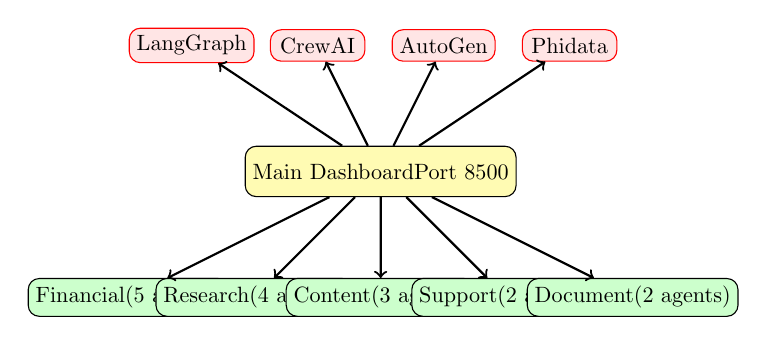
\begin{tikzpicture}[scale=0.8, transform shape,
  box/.style={rectangle, rounded corners, minimum width=2cm, minimum height=0.8cm, text centered, draw=black, fill=blue!20},
  agent/.style={rectangle, rounded corners, minimum width=1.8cm, minimum height=0.6cm, text centered, draw=black, fill=green!20},
  framework/.style={rectangle, rounded corners, minimum width=1.5cm, minimum height=0.5cm, text centered, draw=red, fill=red!10}
]

% Main Dashboard
\node[box, fill=yellow!30] (dashboard) at (0,0) {Main Dashboard\\Port 8500};

% Frameworks
\node[framework] (langgraph) at (-3,2) {LangGraph};
\node[framework] (crewai) at (-1,2) {CrewAI};
\node[framework] (autogen) at (1,2) {AutoGen};
\node[framework] (phidata) at (3,2) {Phidata};

% Agent Categories
\node[agent] (financial) at (-4,-2) {Financial\\(5 agents)};
\node[agent] (research) at (-2,-2) {Research\\(4 agents)};
\node[agent] (content) at (0,-2) {Content\\(3 agents)};
\node[agent] (support) at (2,-2) {Support\\(2 agents)};
\node[agent] (document) at (4,-2) {Document\\(2 agents)};

% Connections
\draw[->, thick] (dashboard) -- (langgraph);
\draw[->, thick] (dashboard) -- (crewai);
\draw[->, thick] (dashboard) -- (autogen);
\draw[->, thick] (dashboard) -- (phidata);

\draw[->, thick] (dashboard) -- (financial);
\draw[->, thick] (dashboard) -- (research);
\draw[->, thick] (dashboard) -- (content);
\draw[->, thick] (dashboard) -- (support);
\draw[->, thick] (dashboard) -- (document);

\end{tikzpicture}
\end{center}
\end{frame}

% Framework Comparison
\begin{frame}{Framework Selection}
\begin{table}
\centering
\small
\begin{tabular}{lll}
\toprule
\textbf{Framework} & \textbf{Best For} & \textbf{Used In} \\
\midrule
\faIcon{project-diagram} LangGraph & Complex workflows & Financial Analysis \\
\faIcon{users} CrewAI & Team collaboration & Stock Analysis \\
\faIcon{comments} AutoGen & Conversations & Research Agent \\
\faIcon{brain} Phidata & Simple assistants & Basic Agents \\
\bottomrule
\end{tabular}
\end{table}

\vspace{0.5cm}

\textbf{Why Multiple Frameworks?}
\begin{itemize}
    \item Each framework has unique strengths
    \item Different use cases require different approaches
    \item Demonstrates interoperability patterns
\end{itemize}
\end{frame}

% Agent Portfolio - Financial
\begin{frame}{Agent Portfolio - Financial Domain}
\begin{columns}
\column{0.6\textwidth}
\textbf{1. Multi-Agent Financial Analysis}
\begin{itemize}
    \item Framework: LangGraph
    \item 7 specialized sub-agents
    \item Conditional routing logic
    \item Port: 8501
\end{itemize}

\textbf{2. Stock Analysis Extended}
\begin{itemize}
    \item Framework: CrewAI
    \item 5 collaborative agents
    \item Technical \& fundamental analysis
    \item Port: 8507
\end{itemize}

\column{0.4\textwidth}
\textbf{3. Finance Advisor}
\begin{itemize}
    \item Personal finance
    \item Port: 8503
\end{itemize}

\textbf{4. Stock Analysis}
\begin{itemize}
    \item Market research
    \item Port: 8509
\end{itemize}

\textbf{5. Competitive Intel}
\begin{itemize}
    \item Business analysis
    \item Port: 8504
\end{itemize}
\end{columns}
\end{frame}

% Agent Portfolio - Research & Content
\begin{frame}{Agent Portfolio - Research \& Content}
\begin{columns}
\column{0.5\textwidth}
\textbf{Research Agents:}
\begin{itemize}
    \item \textbf{ARIA} - AutoGen Research
    \item \textbf{MARIA} - Medical Research
    \item \textbf{Research V2} - General Research
    \item \textbf{Insights Explorer} - Data Insights
\end{itemize}

\column{0.5\textwidth}
\textbf{Content \& Support:}
\begin{itemize}
    \item \textbf{AI Content Creation} - Writing
    \item \textbf{Customer Support} - Helpdesk
    \item \textbf{Support Triage} - Ticket routing
    \item \textbf{Resume Screening} - HR support
\end{itemize}
\end{columns}

\vspace{0.5cm}
\textbf{Document Processing:}
\begin{itemize}
    \item \textbf{Legal Document Review} - Contract analysis (Port: 8501)
    \item \textbf{Handwriting Analysis} - OCR and historical documents (Port: 8516)
\end{itemize}
\end{frame}

% Key Features
\begin{frame}{Key Features}
\begin{columns}
\column{0.5\textwidth}
\textbf{\faIcon{plug} Multi-Provider Support}
\begin{itemize}
    \item OpenAI GPT-4
    \item Anthropic Claude
    \item Google Gemini
    \item HuggingFace Models
    \item Automatic fallback
\end{itemize}

\column{0.5\textwidth}
\textbf{\faIcon{chart-line} Observability}
\begin{itemize}
    \item LangSmith tracing
    \item AgentOps monitoring
    \item Langfuse analytics
    \item Unified logging
    \item Performance tracking
\end{itemize}
\end{columns}

\vspace{0.5cm}

\textbf{\faIcon{docker} Deployment Features}
\begin{itemize}
    \item Containerized microservices
    \item Docker Compose orchestration
    \item Environment-based configuration
    \item Service discovery
    \item Health monitoring
\end{itemize}
\end{frame}

% Technical Implementation
\begin{frame}{Technical Implementation}
\begin{columns}
\column{0.5\textwidth}
\textbf{Project Structure:}
\begin{lstlisting}
training-agentic-ai/
├── agents/
│   ├── multi-agent-financial/
│   ├── stock-analysis-extended/
│   ├── Customer-Support-Triage/
│   └── [13 more agents...]
├── docker-compose.yml
├── requirements.txt
├── .env.example
└── app.py (dashboard)
\end{lstlisting}

\column{0.5\textwidth}
\textbf{Key Technologies:}
\begin{itemize}
    \item \textbf{Frontend}: Streamlit
    \item \textbf{Backend}: Python 3.11+
    \item \textbf{Deployment}: Docker
    \item \textbf{Cache}: Redis
    \item \textbf{Monitoring}: Multi-platform
\end{itemize}

\textbf{Configuration:}
\begin{itemize}
    \item Environment variables
    \item API key management
    \item Service discovery
    \item Port mapping
\end{itemize}
\end{columns}
\end{frame}

% Demo Preparation
\begin{frame}{Demo Overview}
\textbf{What We'll Demonstrate:}

\begin{enumerate}
    \item \textbf{Main Dashboard}
    \begin{itemize}
        \item Agent status monitoring
        \item Service health checks
        \item Quick navigation
    \end{itemize}
    
    \item \textbf{Financial Analysis Agent}
    \begin{itemize}
        \item Stock analysis workflow
        \item Multi-agent collaboration
        \item Report generation
    \end{itemize}
    
    \item \textbf{Customer Support Triage}
    \begin{itemize}
        \item Ticket classification
        \item Priority routing
        \item Response generation
    \end{itemize}
    
    \item \textbf{Research Agent}
    \begin{itemize}
        \item Information gathering
        \item Source citation
        \item Comprehensive reports
    \end{itemize}
\end{enumerate}
\end{frame}

% Access Information
\begin{frame}{System Access}
\begin{center}
\Large
\textbf{Main Dashboard}\\
\vspace{0.3cm}
\faIcon{globe} \texttt{http://localhost:8500}\\
\vspace{1cm}

\normalsize
\begin{tabular}{ll}
\toprule
\textbf{Service} & \textbf{Port} \\
\midrule
Main Dashboard & 8500 \\
Legal Document Review & 8501 \\
Customer Support & 8502 \\
Finance Advisor & 8503 \\
Stock Analysis Extended & 8507 \\
Support Triage & 8506 \\
\bottomrule
\end{tabular}
\end{center}

\vspace{0.5cm}
\textbf{Note:} Ensure Docker services are running via \texttt{docker-compose up}
\end{frame}

% Key Takeaways
\begin{frame}{Key Takeaways}
\begin{itemize}
    \item \textbf{Framework Diversity} - Each framework has its place
    \vspace{0.3cm}
    \item \textbf{Practical Integration} - Multiple frameworks can work together
    \vspace{0.3cm}
    \item \textbf{Production Ready} - Docker deployment with monitoring
    \vspace{0.3cm}
    \item \textbf{Extensible Architecture} - Easy to add new agents
    \vspace{0.3cm}
    \item \textbf{Real-World Applications} - Solving actual business problems
\end{itemize}

\vspace{0.5cm}
\begin{center}
\Large
\textbf{Questions before we start the demo?}
\end{center}
\end{frame}

% Thank You / Demo Time
\begin{frame}
\begin{center}
\Huge
\textbf{Live Demo}\\
\vspace{1cm}
\Large
Let's see the system in action!\\
\vspace{0.5cm}
\normalsize
Starting with the Main Dashboard\\
\texttt{http://localhost:8500}
\end{center}
\end{frame}

\end{document}